
Nous recherchons la meilleure approche de correction parmi les cinq  \'enum\'er\'ees dans le tableau \ref{tab:recapApprocheCorrection}.
Pour ce faire, nous disposons des distributions des distances de correction et de Hamming, des fonctions de repartition de ces distributions et aussi des moyennes de distances de correction et de Hamming associ\'ees aux $k$ cases modifi\'ees. Les distributions des distances de correction et de Hamming sont obtenues avec  $p=0.5$ et la fonction de co\^ut est {\em unitaire}.
Les distributions de distances de chaque approche sont regroup\'ees dans les colonnes $1$ et $2$ dans les figures en annexes \ref{annexe_distribution_0_9}.
%Nous avons montr\'e dans le paragraphe \ref{relationMoyDHmoyDL} que la distance line peut \^etre utilis\'ee comme m\'etrique de comparaison entre deux graphes. Cependant, 
Nous d\'ecidons d'utiliser la moyenne des distances de Hamming pour la comparaison de approches de correction parce qu'il est facile de d\'eterminer le nombre de cases modifi\'ees \'etant donn\'ee que nous connaissons les line-graphes $LG$ et $LG_{k,p}$. 
\newline

%ARRETER ICI
%
%Soit $G_{k,p,\alpha}^{i}$  le $i^{ieme}$  graphe g\'en\'er\'e contenant $k$ cases modifi\'ees la $\alpha^{ieme}$ fois avec la repartition $p=0.5$ des $k$ cases. Nous le notons $G_{k,\alpha}^{i}$ avec $ 0 \le i \le 500$ et $\alpha \le \alpha_{max}$. \\
%Soit $DC_k^i$ le nombre de cases corrig\'ees par l'algorithme de correction pour le graphe $G_{k,\alpha}^{i}$.\\
%$\bar{DC_k^i}$ est la moyenne de $DC_k^i$ pour les $\alpha_{max}$ graphes $G_{k,\alpha}^{i}$.\\ 
%$\bar{DC_k}$ est la moyenne de $\bar{DC_k^i}$ pour $500$ graphes contenant $k$ cases modifi\'ees.\\
%Nous choisissons $\bar{DC_k}$ comme crit\`ere de comparaison des approches de corrections. %parce que A TROUVER 
%\newline
Soit $G_{k,p,\alpha}^{i}$  le $i^{ieme}$  graphe g\'en\'er\'e contenant $k$ cases modifi\'ees la $\alpha^{ieme}$ fois avec la repartition $p=0.5$ des $k$ cases. Nous le notons $G_{k,\alpha}^{i}$ avec $ 0 \le i \le 500$ et $\alpha \le \alpha_{max}$. Le line-graphe de  $G_{k,\alpha}^{i}$ obtenu apr\`es l'algorithme de correction est not\'e $L(G_{k,\alpha}^{i})$. \\
Soit $DH_k^i$ la distance de Hamming entre $LG$ et $L(G_{k,\alpha}^{i})$.  \\
La variable $moy\_DH_{k}^{i}$ est la moyenne de $DH_k^i$ pour les $\alpha_{max}$ graphes $G_{k,\alpha}^{i}$ et la variable $moy\_DH_{k}$ est la moyenne de $moy\_DH_{k}^{i}$ pour $500$ graphes contenant $k$ cases modifi\'ees.
La figure \ref{compareDifferentesMethodesCorrectionSommets_fct_cout_normal_p05} affiche les courbes  des diff\'erents approches de correction pour des distances de Hamming moyenn\'ees $moy\_DH_{k}$ en fonction des $k$ cases modifi\'ees. En ordonn\'e, nous avons le nombre de cases diff\'erentes entre deux line-graphes. 
\newline

% ----------- figure compareDifferentesMethodesCorrectionSommets _fct_cout_normal_p05 ----
%\vspace{-2.0cm}
\begin{figure}[htb!] 
\centering
% a changer par des chemins relatifs
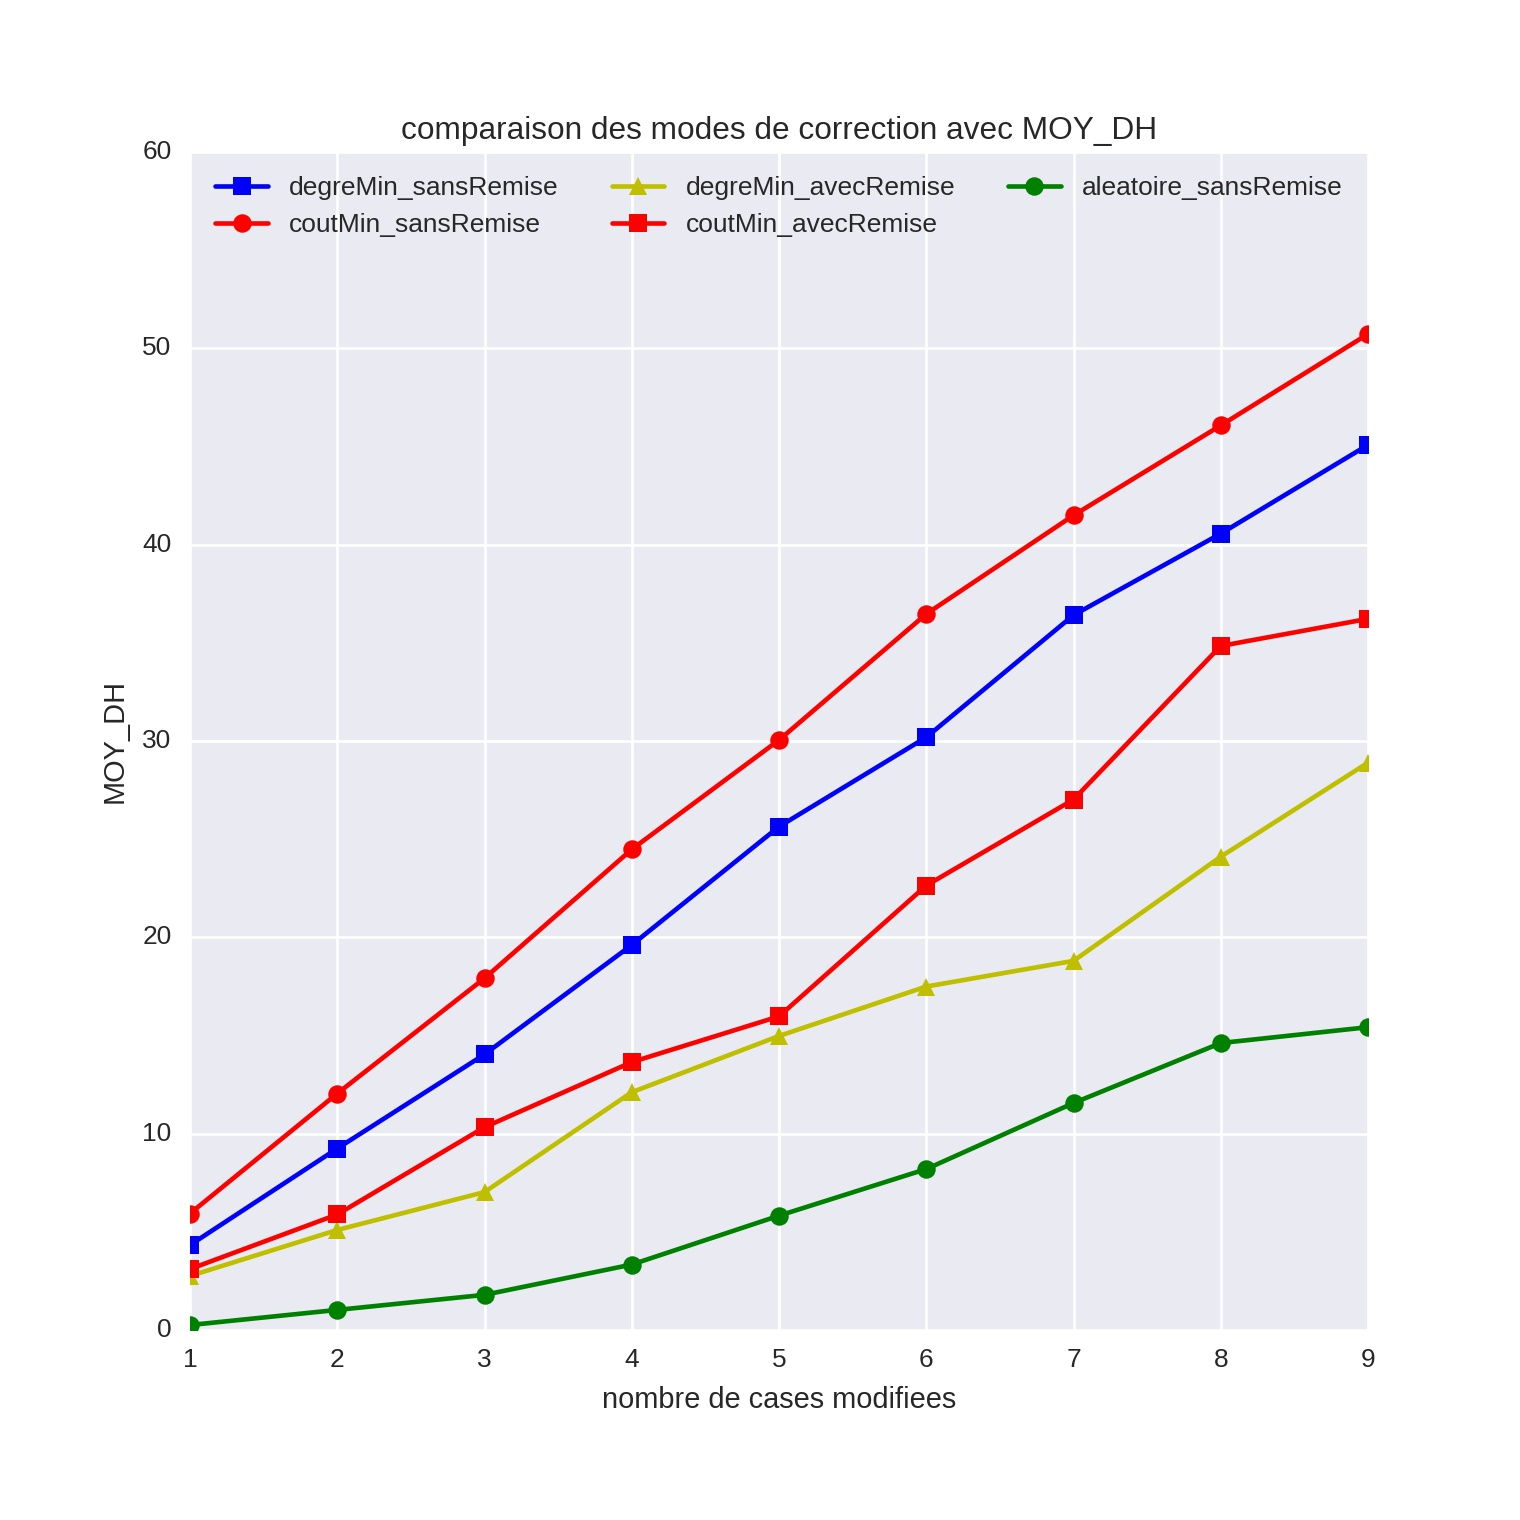
\includegraphics[scale=0.25]{simulation_comparaisonDifferentesMethodes_by_FonctDeCout_unitaire_500G_p_correl_05.jpeg}
\caption{ Comparaison des diff\'erentes approches de correction de sommets pour $k \in \{1,\cdots,9\}$ cases modifi\'ees. 
Les courbes en bleu carr\'e : approche degr\'e minimum sans remise (2a), 
			rouge carr\'ee : approche co\^ut minimum avec remise (1b), 
			rouge rond : approche co\^ut minimum sans remise (2b), 
			vert rond : approche al\'eatoire sans remise (2c) et 
			jaune triangle : approche degr\'e minimum avec remise (1a) 
}
\label{compareDifferentesMethodesCorrectionSommets_fct_cout_normal_p05} 
\end{figure}
\FloatBarrier
% ----------- figure compareDifferentesMethodesCorrectionSommets _fct_cout_normal_p05 ----


Consid\'erons des courbes associ\'ees aux approches $(2b)$, $(2c)$ et $(1b)$. 
En choisissant les nombres de cases modifi\'ees $k \in \{4, 8\}$, nous avons $moy\_DH_{k,p} \in \{4,15\}$ cases pour l'approche $(2c)$, $moy\_DH_{k,p} \in \{13, 36\}$ cases  pour l'approche $(1b)$ et $moy\_DH_{k,p} \in \{25, 46\}$ cases  pour l'approche $(2b)$.
Pour $k=4$ cases modifi\'ees, l'approche $(1b)$  modifie, en moyenne, $9$ cases de plus que l'approche $(2c)$. En revanche, ce nombre moyen de cases modifi\'ees augmente \`a $21$ cases quand $k=8$. 
De m\^eme, l'approche $(2b)$ modifie $12$ cases de plus que l'approche $(1b)$ pour $k=4$ cases modifi\'ees et $10$ cases pour $k=8$ cases.
L'approche  $(2c)$ donne de meilleures r\'esultats par rapport aux approches $(1b)$ et $(2b)$.
\newline


% conclusion
{\bf Conclusion} : l'approche {\em al\'eatoire sans remise} propose de meilleurs r\'esultats que les approches $(2a)$, $(2b)$, $(1a)$ et $(1b)$ parce que les distances de correction sont minimales pour toute valeur de $k$ comme le montre la figure \ref{compareDifferentesMethodesCorrectionSommets_fct_cout_normal_p05}.
Nous retenons, pour la suite,  l'approche {\em al\'eatoire sans remise}  comme l'approche de correction des sommets de $\cal C$, sommets n'appartenant \`a aucune couverture.
%D'autre part, ce r\'esultat a \'et\'e obtenu avec la fonction de co\^ut {\em unitaire}.



